  

\section{Joachimsthal's Integral}

\textcolor{red}{ron: introduzir e uniformizar notacao}


\begin{proposition}\label{prop:invariant_joachim} Consider an ellipse $\mathcal{E}$ defined by $\langle A P,P\rangle=1$. Let $u$ be an inward unit vector in the direction of the billiard orbit passing through the point $P_0\in\mathcal{E} $. Let $T(P_1,u)=(P_2,v)$ the billiard map as shown in   \cref{fig:appC-joachim}.
	Then 
	\[  \langle A P_1,u\rangle =  -\langle A P_2,u\rangle=  \langle A P_2,v\rangle  \]
	
	\end{proposition}

%trim=left bottom right top
\begin{figure}[H]
	\begin{center}
 %	\def\svgwidth{0.75\textwidth}
	 %	\input{pics_tex/joachim.eps_tex}
	 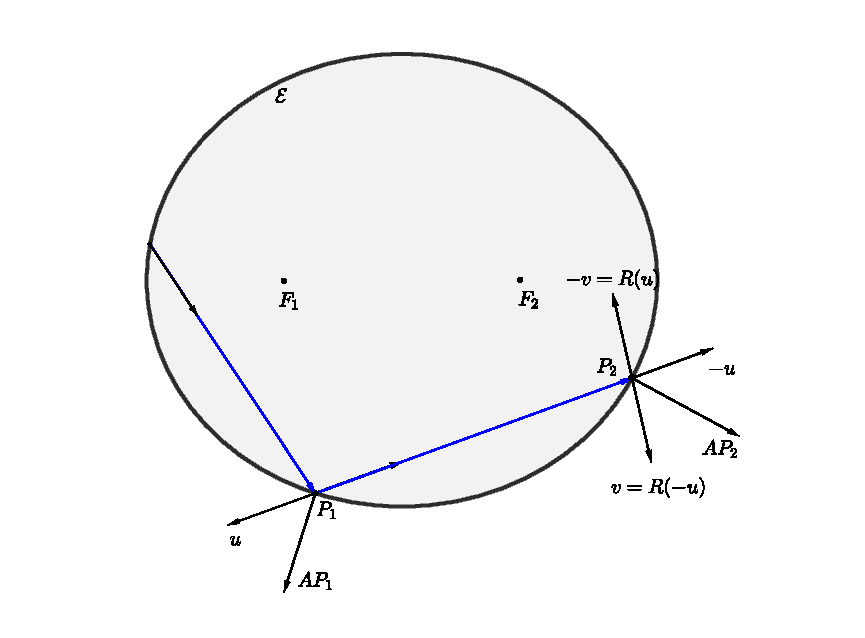
\includegraphics[scale=0.6]{pics_appC_050_joachimstall.pdf}
	 %	 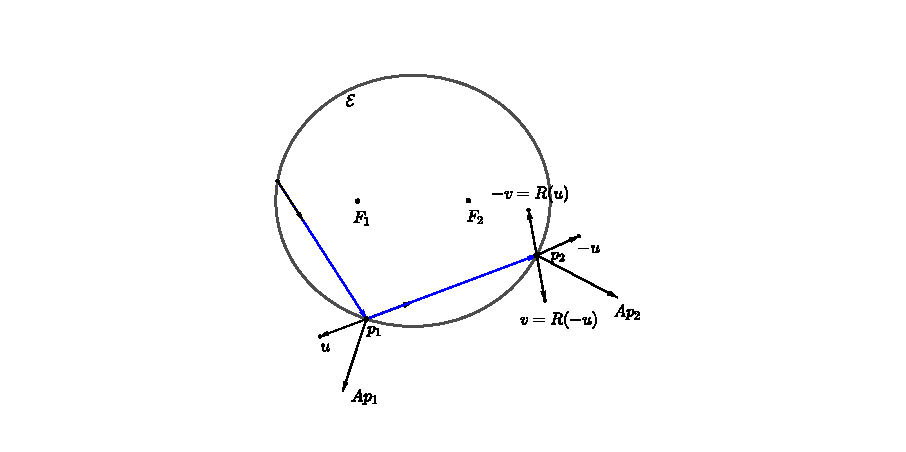
\includegraphics[scale=0.9]{pics_tex/joachimstall.pdf}
		\caption {Joachimsthal's first integral  $\langle AP_1,u\rangle $ is T-invariant.}
		 \label{fig:appC-joachim}
	\end{center}
\end{figure}

\begin{proof} The tangent space  $T_{p}\mathcal{E}$ is formed of the vectors $u$ such that $ \langle A P,u\rangle =0.$ Therefore $AP$ is a normal vector to the ellipse at the point $P$. The vector $u$ is proportional to $P_2-P_1$.
	
	Therefore,
	\begin{align*}  \langle AP_1+AP_2 , P_2-P_1\rangle &= \langle AP_1  , P_2 \rangle + \langle AP_2  , P_1 \rangle  - \langle AP_1  , P_1 \rangle + \langle AP_2  , P_2 \rangle \\
	&= \langle  P_1  , AP_2 \rangle - \langle AP_2  , P_1 \rangle =0. 
	\end{align*}
	Then,
	\[ \langle AP_1 , u\rangle =\langle  AP_2 ,-u\rangle  =  \langle  AP_2 ,R(-u)\rangle  =  \langle  AP_2, v\rangle \]
	\end{proof}